\section{Controlling}

The main task of the project requires the robot to move with the highest possible speed.
On the other hand the robot should be able to move at a speed that induces as little drift as possible and reduces the risk of errors when hitting an obstacle.
And lastly, the vision would have to identify objects from further away, increasing the difficulty of implementation and recognition.
Thus, a balance in the velocities have to be found.\\

The implemented controllers consisted of a forward movement controller, a turn controller and a wall alignment controller.
By embedding them in an adapter pattern it was possible to render their usage very versatile (see figure \ref{fig:arch_controller}).
Every controller inherited hereby a controller base which defined an interface that updated the logic and returned a Twist
(A Twist is one of many ros pre-baked data structures that can be sent as a message. 
It stores a position and a rotation). 
The adapter combines all received Twists to one Twist, entrusting that no contradictions occur.
A top logic has to ensure that the right controllers are activated and deactivated.
This can be done by activating and deactivating each controller.
Controllers like the turn and the forward movement controller respond with a message as soon as they have stopped or finished their activity.\\

\begin{figure}[h]
\begin{center}
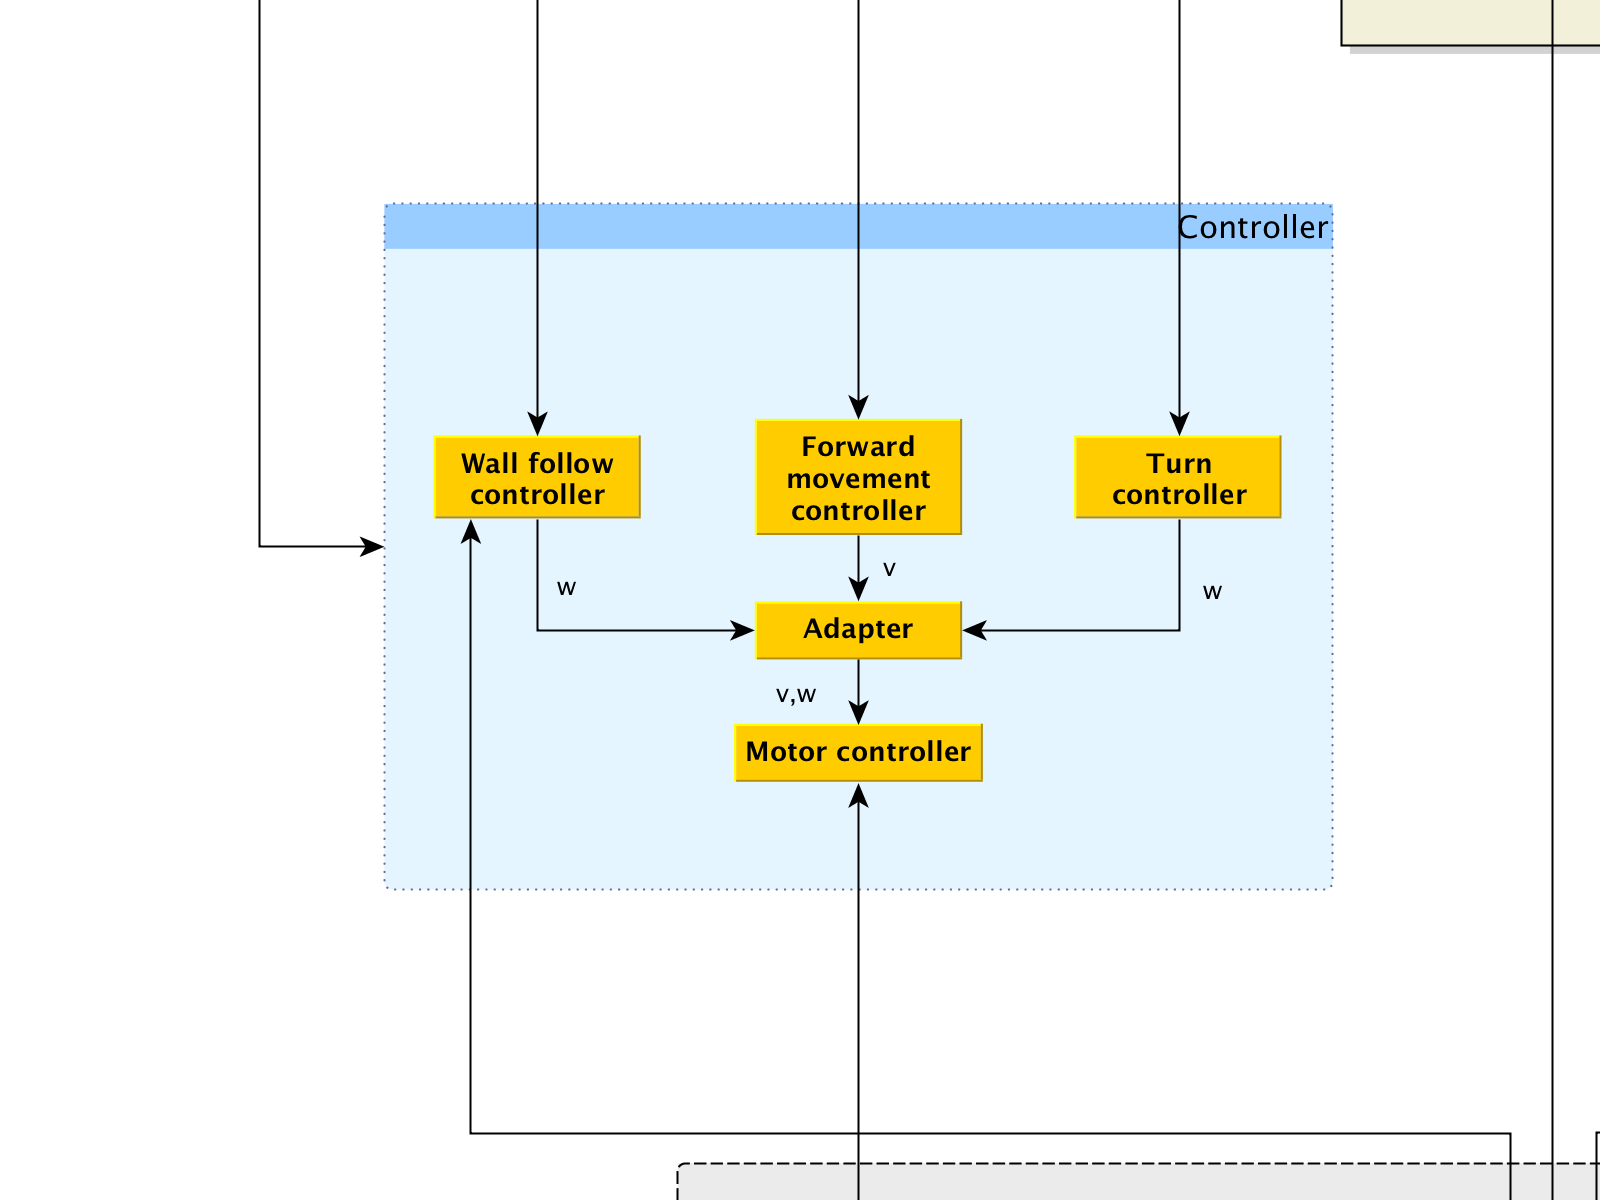
\includegraphics[width=0.6\textwidth]{figures/arch_controller.png}
\end{center}
\caption{Architecture of the controller package}
\label{fig:arch_controller}
\end{figure}

\subsection{Motor controller}

Due to internal motor difference, it is not sufficient to control the motors directly.
Otherwise the robot would move in an arch, one motor rotating slower than the other.
To compensate for that and to also be able to input linear and angular velocities, a PID controller was used. 
This enabled the robot to drive in a stable straight line.

The motors itself have a static resistance, that have to be overcome whenever the motors should transition from idling to rotating.
Overcoming these static resistance could be described by constants (for each motor one) $K_{power}$, that were added to the result of the PID results.
As soon as the static resistance has been overcome and the motor is rotating, the constant $K_{power}$ can be reduced to a value that sustains rotation: $K_{sustain}$.
This behavior results in a spiked motor control output as can be seen in figure \ref{fig:pwm_spiker}.
Although movement without spiking is possible due to the accumulating behavior of the PID controller too, it ensures responsive controlling and avoids the necessecity of increasing the gains which can easily result in overshoots.

\begin{figure}[h]
\begin{center}
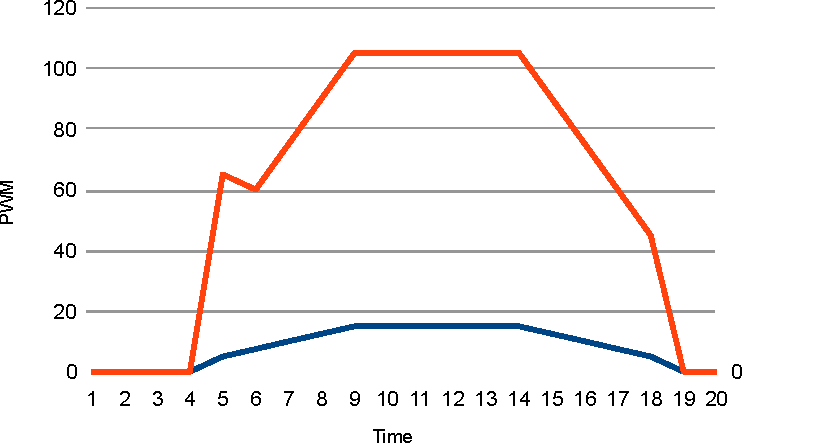
\includegraphics[width=0.6\textwidth]{figures/pwm_spike.pdf}
\end{center}
\caption{PWM Spiking for initial motor rotation attempt}
\label{fig:pwm_spiker}
\end{figure}

\subsection{Wall alignment}

The wall allignment controller (see figure \ref{fig:arch_controller}) uses the IR sensors to measure the distances from the robot to the walls, and works as follows: if both walls are close to the robot (distance < 0.4 m), then keep the robot aligned to the center between both walls.
Otherwise control only by the next closest wall, or if no wall is present, do not align.